\documentclass{beamer}
% Setup appearance:
\usetheme{Marburg} 

\usepackage{color} % It may be necessary to set PCTeX or whatever program you are using to output a .pdf instead of a .dvi file in order to see color on your screen.
\usepackage{graphicx} 

\usepackage[spanish]{babel}
\usepackage[latin1]{inputenc}
\usepackage{amsmath}
\usepackage{mathtools}
\usepackage{calrsfs}
\usepackage{cases}
\usepackage{hyperref}

\usepackage{tikz}
\usetikzlibrary{arrows}
\tikzstyle{block}=[draw opacity=0.7,line width=1.4cm]


% Author, Title, etc.

\title[] 
{%
  Programaci�n de la EDU-CIAA en lenguaje C (\textit{sin RTOS})\\ 
 %5ta ESE - Horco Molle 2015 %
}
	
\author[]
{
Bioing.~Juan~Manuel Reta \\ Mgt Eduardo Filomena~\
}

%\insertshortdate
\date[2015]
{}


% The main document

\begin{document}

\begin{frame}
% \begin{center}

%\end{center}
  \titlepage
\begin{center}
  
	
\includegraphics[height=1cm]{Imagenes/logo_ruse}
\hspace{1cm}
	
\includegraphics[height=1cm]{Imagenes/acse}
\end{center}

\end{frame}

\section{Firmware}

\begin{frame}{Estructura Repositorio}

\begin{center}
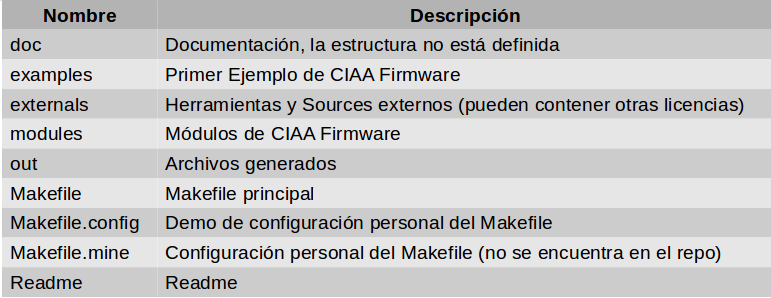
\includegraphics[height=3.5cm]{Imagenes/estructura_repo}
\end{center}
\vspace{0.2 cm}
\begin{center}
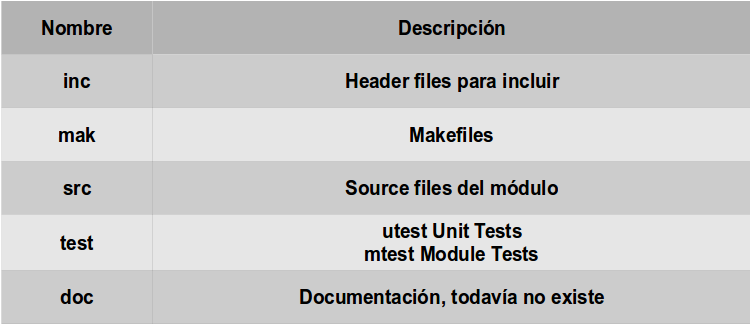
\includegraphics[height=3.5cm]{Imagenes/estructura_modulos}
\end{center}
\end{frame}

\section{Estructura Firmware}
\begin{frame}{Estructura Firmware}

\begin{center}
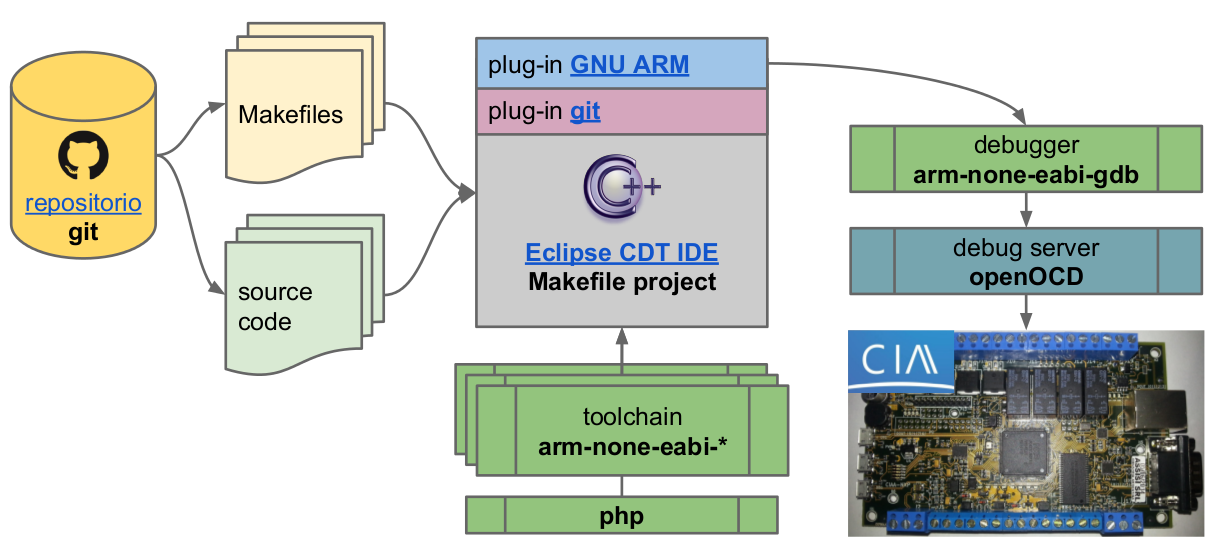
\includegraphics[height=4.5cm]{Imagenes/fimrware}
\end{center}
\begin{flushright}
{\footnotesize Fig: Ing. Pablo Ridolfi}
\end{flushright}
\end{frame}

\section{ToolChain}

\section{Make}

\section{Ejercitaci�n}

\begin{frame}{}
\begin{center}

\includegraphics[height=4cm]{Imagenes/confucio}
\end{center}
\vspace{1cm}
\begin{flushright}
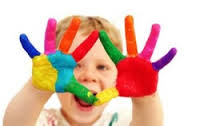
\includegraphics[height=2cm]{Imagenes/apredizaje}
\end{flushright}
\end{frame}


\begin{frame}{Ejercitacio 1 (Blinking)}

\begin{center}
\textbf{Explore las potencialidades de la Juntura PN}
\end{center}
\begin{center}
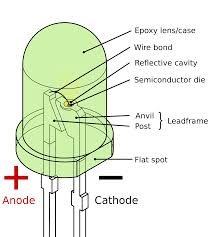
\includegraphics[height=5cm]{Imagenes/led}
\end{center}

\end{frame}

\end{document}
